% Options for packages loaded elsewhere
\PassOptionsToPackage{unicode}{hyperref}
\PassOptionsToPackage{hyphens}{url}
\PassOptionsToPackage{dvipsnames,svgnames,x11names}{xcolor}
%
\documentclass[
  letterpaper,
  DIV=11,
  numbers=noendperiod]{scrreprt}

\usepackage{amsmath,amssymb}
\usepackage{iftex}
\ifPDFTeX
  \usepackage[T1]{fontenc}
  \usepackage[utf8]{inputenc}
  \usepackage{textcomp} % provide euro and other symbols
\else % if luatex or xetex
  \usepackage{unicode-math}
  \defaultfontfeatures{Scale=MatchLowercase}
  \defaultfontfeatures[\rmfamily]{Ligatures=TeX,Scale=1}
\fi
\usepackage{lmodern}
\ifPDFTeX\else  
    % xetex/luatex font selection
\fi
% Use upquote if available, for straight quotes in verbatim environments
\IfFileExists{upquote.sty}{\usepackage{upquote}}{}
\IfFileExists{microtype.sty}{% use microtype if available
  \usepackage[]{microtype}
  \UseMicrotypeSet[protrusion]{basicmath} % disable protrusion for tt fonts
}{}
\makeatletter
\@ifundefined{KOMAClassName}{% if non-KOMA class
  \IfFileExists{parskip.sty}{%
    \usepackage{parskip}
  }{% else
    \setlength{\parindent}{0pt}
    \setlength{\parskip}{6pt plus 2pt minus 1pt}}
}{% if KOMA class
  \KOMAoptions{parskip=half}}
\makeatother
\usepackage{xcolor}
\setlength{\emergencystretch}{3em} % prevent overfull lines
\setcounter{secnumdepth}{5}
% Make \paragraph and \subparagraph free-standing
\ifx\paragraph\undefined\else
  \let\oldparagraph\paragraph
  \renewcommand{\paragraph}[1]{\oldparagraph{#1}\mbox{}}
\fi
\ifx\subparagraph\undefined\else
  \let\oldsubparagraph\subparagraph
  \renewcommand{\subparagraph}[1]{\oldsubparagraph{#1}\mbox{}}
\fi

\usepackage{color}
\usepackage{fancyvrb}
\newcommand{\VerbBar}{|}
\newcommand{\VERB}{\Verb[commandchars=\\\{\}]}
\DefineVerbatimEnvironment{Highlighting}{Verbatim}{commandchars=\\\{\}}
% Add ',fontsize=\small' for more characters per line
\usepackage{framed}
\definecolor{shadecolor}{RGB}{241,243,245}
\newenvironment{Shaded}{\begin{snugshade}}{\end{snugshade}}
\newcommand{\AlertTok}[1]{\textcolor[rgb]{0.68,0.00,0.00}{#1}}
\newcommand{\AnnotationTok}[1]{\textcolor[rgb]{0.37,0.37,0.37}{#1}}
\newcommand{\AttributeTok}[1]{\textcolor[rgb]{0.40,0.45,0.13}{#1}}
\newcommand{\BaseNTok}[1]{\textcolor[rgb]{0.68,0.00,0.00}{#1}}
\newcommand{\BuiltInTok}[1]{\textcolor[rgb]{0.00,0.23,0.31}{#1}}
\newcommand{\CharTok}[1]{\textcolor[rgb]{0.13,0.47,0.30}{#1}}
\newcommand{\CommentTok}[1]{\textcolor[rgb]{0.37,0.37,0.37}{#1}}
\newcommand{\CommentVarTok}[1]{\textcolor[rgb]{0.37,0.37,0.37}{\textit{#1}}}
\newcommand{\ConstantTok}[1]{\textcolor[rgb]{0.56,0.35,0.01}{#1}}
\newcommand{\ControlFlowTok}[1]{\textcolor[rgb]{0.00,0.23,0.31}{#1}}
\newcommand{\DataTypeTok}[1]{\textcolor[rgb]{0.68,0.00,0.00}{#1}}
\newcommand{\DecValTok}[1]{\textcolor[rgb]{0.68,0.00,0.00}{#1}}
\newcommand{\DocumentationTok}[1]{\textcolor[rgb]{0.37,0.37,0.37}{\textit{#1}}}
\newcommand{\ErrorTok}[1]{\textcolor[rgb]{0.68,0.00,0.00}{#1}}
\newcommand{\ExtensionTok}[1]{\textcolor[rgb]{0.00,0.23,0.31}{#1}}
\newcommand{\FloatTok}[1]{\textcolor[rgb]{0.68,0.00,0.00}{#1}}
\newcommand{\FunctionTok}[1]{\textcolor[rgb]{0.28,0.35,0.67}{#1}}
\newcommand{\ImportTok}[1]{\textcolor[rgb]{0.00,0.46,0.62}{#1}}
\newcommand{\InformationTok}[1]{\textcolor[rgb]{0.37,0.37,0.37}{#1}}
\newcommand{\KeywordTok}[1]{\textcolor[rgb]{0.00,0.23,0.31}{#1}}
\newcommand{\NormalTok}[1]{\textcolor[rgb]{0.00,0.23,0.31}{#1}}
\newcommand{\OperatorTok}[1]{\textcolor[rgb]{0.37,0.37,0.37}{#1}}
\newcommand{\OtherTok}[1]{\textcolor[rgb]{0.00,0.23,0.31}{#1}}
\newcommand{\PreprocessorTok}[1]{\textcolor[rgb]{0.68,0.00,0.00}{#1}}
\newcommand{\RegionMarkerTok}[1]{\textcolor[rgb]{0.00,0.23,0.31}{#1}}
\newcommand{\SpecialCharTok}[1]{\textcolor[rgb]{0.37,0.37,0.37}{#1}}
\newcommand{\SpecialStringTok}[1]{\textcolor[rgb]{0.13,0.47,0.30}{#1}}
\newcommand{\StringTok}[1]{\textcolor[rgb]{0.13,0.47,0.30}{#1}}
\newcommand{\VariableTok}[1]{\textcolor[rgb]{0.07,0.07,0.07}{#1}}
\newcommand{\VerbatimStringTok}[1]{\textcolor[rgb]{0.13,0.47,0.30}{#1}}
\newcommand{\WarningTok}[1]{\textcolor[rgb]{0.37,0.37,0.37}{\textit{#1}}}

\providecommand{\tightlist}{%
  \setlength{\itemsep}{0pt}\setlength{\parskip}{0pt}}\usepackage{longtable,booktabs,array}
\usepackage{calc} % for calculating minipage widths
% Correct order of tables after \paragraph or \subparagraph
\usepackage{etoolbox}
\makeatletter
\patchcmd\longtable{\par}{\if@noskipsec\mbox{}\fi\par}{}{}
\makeatother
% Allow footnotes in longtable head/foot
\IfFileExists{footnotehyper.sty}{\usepackage{footnotehyper}}{\usepackage{footnote}}
\makesavenoteenv{longtable}
\usepackage{graphicx}
\makeatletter
\def\maxwidth{\ifdim\Gin@nat@width>\linewidth\linewidth\else\Gin@nat@width\fi}
\def\maxheight{\ifdim\Gin@nat@height>\textheight\textheight\else\Gin@nat@height\fi}
\makeatother
% Scale images if necessary, so that they will not overflow the page
% margins by default, and it is still possible to overwrite the defaults
% using explicit options in \includegraphics[width, height, ...]{}
\setkeys{Gin}{width=\maxwidth,height=\maxheight,keepaspectratio}
% Set default figure placement to htbp
\makeatletter
\def\fps@figure{htbp}
\makeatother
% definitions for citeproc citations
\NewDocumentCommand\citeproctext{}{}
\NewDocumentCommand\citeproc{mm}{%
  \begingroup\def\citeproctext{#2}\cite{#1}\endgroup}
\makeatletter
 % allow citations to break across lines
 \let\@cite@ofmt\@firstofone
 % avoid brackets around text for \cite:
 \def\@biblabel#1{}
 \def\@cite#1#2{{#1\if@tempswa , #2\fi}}
\makeatother
\newlength{\cslhangindent}
\setlength{\cslhangindent}{1.5em}
\newlength{\csllabelwidth}
\setlength{\csllabelwidth}{3em}
\newenvironment{CSLReferences}[2] % #1 hanging-indent, #2 entry-spacing
 {\begin{list}{}{%
  \setlength{\itemindent}{0pt}
  \setlength{\leftmargin}{0pt}
  \setlength{\parsep}{0pt}
  % turn on hanging indent if param 1 is 1
  \ifodd #1
   \setlength{\leftmargin}{\cslhangindent}
   \setlength{\itemindent}{-1\cslhangindent}
  \fi
  % set entry spacing
  \setlength{\itemsep}{#2\baselineskip}}}
 {\end{list}}
\usepackage{calc}
\newcommand{\CSLBlock}[1]{\hfill\break\parbox[t]{\linewidth}{\strut\ignorespaces#1\strut}}
\newcommand{\CSLLeftMargin}[1]{\parbox[t]{\csllabelwidth}{\strut#1\strut}}
\newcommand{\CSLRightInline}[1]{\parbox[t]{\linewidth - \csllabelwidth}{\strut#1\strut}}
\newcommand{\CSLIndent}[1]{\hspace{\cslhangindent}#1}

\usepackage{makeidx}
\makeindex
\KOMAoption{captions}{tableheading}
\makeatletter
\@ifpackageloaded{tcolorbox}{}{\usepackage[skins,breakable]{tcolorbox}}
\@ifpackageloaded{fontawesome5}{}{\usepackage{fontawesome5}}
\definecolor{quarto-callout-color}{HTML}{909090}
\definecolor{quarto-callout-note-color}{HTML}{0758E5}
\definecolor{quarto-callout-important-color}{HTML}{CC1914}
\definecolor{quarto-callout-warning-color}{HTML}{EB9113}
\definecolor{quarto-callout-tip-color}{HTML}{00A047}
\definecolor{quarto-callout-caution-color}{HTML}{FC5300}
\definecolor{quarto-callout-color-frame}{HTML}{acacac}
\definecolor{quarto-callout-note-color-frame}{HTML}{4582ec}
\definecolor{quarto-callout-important-color-frame}{HTML}{d9534f}
\definecolor{quarto-callout-warning-color-frame}{HTML}{f0ad4e}
\definecolor{quarto-callout-tip-color-frame}{HTML}{02b875}
\definecolor{quarto-callout-caution-color-frame}{HTML}{fd7e14}
\makeatother
\makeatletter
\@ifpackageloaded{bookmark}{}{\usepackage{bookmark}}
\makeatother
\makeatletter
\@ifpackageloaded{caption}{}{\usepackage{caption}}
\AtBeginDocument{%
\ifdefined\contentsname
  \renewcommand*\contentsname{Table of contents}
\else
  \newcommand\contentsname{Table of contents}
\fi
\ifdefined\listfigurename
  \renewcommand*\listfigurename{List of Figures}
\else
  \newcommand\listfigurename{List of Figures}
\fi
\ifdefined\listtablename
  \renewcommand*\listtablename{List of Tables}
\else
  \newcommand\listtablename{List of Tables}
\fi
\ifdefined\figurename
  \renewcommand*\figurename{Figure}
\else
  \newcommand\figurename{Figure}
\fi
\ifdefined\tablename
  \renewcommand*\tablename{Table}
\else
  \newcommand\tablename{Table}
\fi
}
\@ifpackageloaded{float}{}{\usepackage{float}}
\floatstyle{ruled}
\@ifundefined{c@chapter}{\newfloat{codelisting}{h}{lop}}{\newfloat{codelisting}{h}{lop}[chapter]}
\floatname{codelisting}{Listing}
\newcommand*\listoflistings{\listof{codelisting}{List of Listings}}
\makeatother
\makeatletter
\makeatother
\makeatletter
\@ifpackageloaded{caption}{}{\usepackage{caption}}
\@ifpackageloaded{subcaption}{}{\usepackage{subcaption}}
\makeatother
\makeatletter
\@ifpackageloaded{tikz}{}{\usepackage{tikz}}
\makeatother
        \newcommand*\circled[1]{\tikz[baseline=(char.base)]{
          \node[shape=circle,draw,inner sep=1pt] (char) {{\scriptsize#1}};}}  
                  
\ifLuaTeX
  \usepackage{selnolig}  % disable illegal ligatures
\fi
\usepackage{bookmark}

\IfFileExists{xurl.sty}{\usepackage{xurl}}{} % add URL line breaks if available
\urlstyle{same} % disable monospaced font for URLs
\hypersetup{
  pdftitle={From Code to Commerce: PyTorch Deep Dive into AI, Mathematics, and Business Tactics},
  pdfauthor={Ivan Jacobs},
  colorlinks=true,
  linkcolor={blue},
  filecolor={Maroon},
  citecolor={Blue},
  urlcolor={Blue},
  pdfcreator={LaTeX via pandoc}}

\title{From Code to Commerce: PyTorch Deep Dive into AI, Mathematics,
and Business Tactics}
\author{Ivan Jacobs}
\date{2025-01-12}

\begin{document}
\maketitle

\renewcommand*\contentsname{Table of contents}
{
\hypersetup{linkcolor=}
\setcounter{tocdepth}{2}
\tableofcontents
}
\bookmarksetup{startatroot}

\chapter*{Preface}\label{preface}
\addcontentsline{toc}{chapter}{Preface}

\markboth{Preface}{Preface}

In the vast realm of technology, where innovation and business strategy
converge, a new frontier is emerging -- one defined by the symbiotic
relationship between code and commerce. Welcome to ``From Code to
Commerce: PyTorch Deep Dive into AI, Mathematics, and Business
Tactics.'' In this transformative journey, we embark on a quest to
demystify the complexities of Artificial Intelligence (AI) by delving
into the depths of PyTorch, a powerful tool that seamlessly intertwines
the intricacies of code, the elegance of mathematics, and the pragmatism
of business strategy.

Artificial intelligence (AI) has become an integral part of our daily
lives, transforming the way we live, work, and interact with each other.
The rapid advancements in AI technology have made it possible to
automate complex tasks, make informed decisions, and create innovative
products and services.

As the world becomes increasingly entwined with AI, there is a growing
need for a holistic understanding of this formidable technology. This
book is not just a guide; it's a roadmap that navigates the reader
through the evolving landscape of AI, from its theoretical foundations
to tangible applications in the business world.

Our journey begins with a deep dive into PyTorch, a versatile and
dynamic framework that has become synonymous with AI innovation. Through
hands-on projects, meticulously worked out in PyTorch, we bridge the gap
between theory and practice, empowering readers to grasp the nuances of
AI implementation. Each project serves as a canvas where code is an
artist's brush, crafting intelligent solutions to real-world challenges.

But this book is more than just a coding manual. It is a mathematical
odyssey where the theoretical underpinnings of AI are illuminated. For
every project, we unravel the mathematical proofs with clarity and
precision, providing a comprehensive understanding of the algorithms and
models that breathe life into artificial intelligence.

Beyond the realms of code and mathematics, ``From Code to Commerce''
introduces a crucial third dimension -- the strategic integration of AI
into the fabric of commerce. Each project is not merely an academic
exercise but a strategic venture with a concrete business strategy. From
conceptualization to implementation, we explore the tactical
considerations that transform AI projects into thriving ventures.

Whether you are a seasoned developer, a curious entrepreneur, or a
business leader seeking to harness the power of AI, this book is your
companion in the journey from code to commerce. The fusion of PyTorch
proficiency, mathematical insight, and business acumen creates a synergy
that goes beyond the traditional boundaries of AI literature. Join us as
we unravel the potential of AI, one line of code, one mathematical
proof, and one strategic business plan at a time. Welcome to the
intersection of innovation and commerce -- where the future is not just
imagined but coded, calculated, and strategically conquered.

\bookmarksetup{startatroot}

\chapter*{Introduction}\label{introduction}
\addcontentsline{toc}{chapter}{Introduction}

\markboth{Introduction}{Introduction}

\part{AI-Driven Trading}

\textbf{Introduction to AI-Driven Trading: Unleashing the Future of
Financial Markets}

In the fast-paced realm of financial markets, the convergence of
artificial intelligence (AI) and trading has ushered in a new era of
innovation, transforming the landscape of investment and risk
management. Welcome to the world of AI-driven trading, where algorithms,
machine learning, and sophisticated models are reshaping the way
financial decisions are made, offering unparalleled speed, accuracy, and
adaptability.

The traditional paradigms of trading, once dominated by human intuition
and analysis, are now being augmented and, in some cases, replaced by AI
technologies. These intelligent systems have the capacity to ingest vast
amounts of data, analyze market trends in real-time, and execute trades
with precision that surpasses human capabilities. The result is a
seismic shift in the dynamics of financial markets, where algorithms
operate at speeds inconceivable to the human mind, making split-second
decisions that can define success in a highly competitive environment.

AI-driven trading is not merely a technological trend; it represents a
paradigm shift in the philosophy of trading strategies. From predictive
analytics to machine learning models, AI equips traders with tools to
not only interpret historical data but also forecast future market
movements. The ability to adapt to changing conditions, identify
emerging patterns, and execute trades with remarkable efficiency gives
AI-driven trading a distinct edge in the ever-evolving financial
landscape.

This introduction marks the threshold of a comprehensive exploration
into the multifaceted dimensions of AI-driven trading. Over the course
of this journey, we will unravel the intricacies of algorithmic trading,
exploring how AI enhances decision-making processes and risk management.
From quantitative trading strategies to the ethical considerations
surrounding autonomous trading systems, each chapter will illuminate a
facet of the AI revolution that is transforming the financial world.

Whether you are a seasoned trader seeking to harness the power of AI or
an enthusiast eager to understand the future of financial markets, this
exploration into AI-driven trading promises to be enlightening and
insightful. Join us as we navigate the fascinating intersection of
artificial intelligence and finance, where algorithms don't just crunch
numbers but redefine the very nature of trading itself. Welcome to the
frontier of AI-driven trading---an intelligent evolution that is
reshaping the future of financial markets.

AI-driven trading, also known as automated trading or algorithmic
trading, refers to the use of artificial intelligence (AI) and machine
learning (ML) techniques to execute trades automatically in financial
markets. The goal of AI-driven trading is to make trades more
efficiently and effectively than human traders, by leveraging the power
of AI to analyze market data, identify patterns, and make decisions in
real-time.

\section*{Types of AI-driven trading
strategies:}\label{types-of-ai-driven-trading-strategies}
\addcontentsline{toc}{section}{Types of AI-driven trading strategies:}

\markright{Types of AI-driven trading strategies:}

There are several ways in which AI can be used in trading, including:

\begin{enumerate}
\def\labelenumi{\arabic{enumi}.}
\item
  Predictive modeling: AI algorithms can be trained on historical market
  data to predict future price movements and identify potential trading
  opportunities.
\item
  High-frequency trading: AI can be used to execute trades at extremely
  high speeds, allowing for rapid execution of trades and taking
  advantage of small price discrepancies across different markets.
\item
  Portfolio optimization: AI can be used to optimize a portfolio of
  assets by identifying the most profitable trades and adjusting the
  portfolio in real-time to maximize returns.
\item
  Risk management: AI can be used to monitor and manage risk in
  real-time, by identifying potential risks and adjusting trades
  accordingly.
\item
  Natural language processing: AI can be used to analyze and understand
  natural language news and social media feeds to identify potential
  trading opportunities.
\item
  Sentiment analysis: AI can be used to analyze market sentiment and
  identify potential trading opportunities based on market sentiment.
\item
  Technical analysis: AI can be used to analyze technical indicators and
  identify potential trading opportunities based on chart patterns and
  other technical analysis tools.
\item
  Machine learning: AI can be used to learn from historical market data
  and improve trading strategies over time.
\item
  Neural networks: AI can be used to create neural networks that can
  learn and improve over time, allowing for more complex and
  sophisticated trading strategies.
\item
  Robotic trading: AI can be used to create automated trading systems
  that can execute trades automatically based on predefined rules and
  strategies.
\end{enumerate}

\section*{Advantages of AI-driven
trading:}\label{advantages-of-ai-driven-trading}
\addcontentsline{toc}{section}{Advantages of AI-driven trading:}

\markright{Advantages of AI-driven trading:}

AI-driven trading can provide several advantages, including faster
execution times, improved accuracy, and the ability to analyze vast
amounts of data.

The benefits of AI-driven trading include:

\begin{enumerate}
\def\labelenumi{\arabic{enumi}.}
\item
  Increased speed and accuracy: AI algorithms can analyze and execute
  trades faster and more accurately than human traders, allowing for
  faster and more profitable trades.
\item
  Emotional detachment: AI algorithms are not subject to the same
  emotional biases as human traders, allowing for more objective and
  rational trading decisions.
\item
  24/7 Trading: AI algorithms can monitor markets 24/7 and execute
  trades at any time, even when markets are closed.
\item
  Scalability: AI algorithms can handle large amounts of data and
  execute trades quickly and efficiently, allowing for scalable trading
  strategies.
\item
  Diversification: AI algorithms can identify and execute trades in
  multiple markets and asset classes, allowing for diversification of
  the portfolio.
\item
  Risk management: AI algorithms can monitor and manage risk in
  real-time, allowing for more effective risk management.
\item
  Improved decision making: AI algorithms can analyze large amounts of
  data and make decisions based on patterns and trends, allowing for
  more informed trading decisions.
\item
  Cost savings: AI algorithms can reduce trading costs by automating
  tasks and improving efficiency.
\item
  Increased efficiency: AI algorithms can automate routine tasks and
  improve the overall efficiency of trading operations.
\item
  Competitive advantage: AI-driven trading can provide a competitive
  advantage by allowing firms to make faster and more accurate trading
  decisions, and to execute trades more efficiently than their
  competitors.
\end{enumerate}

\section*{Challenges of AI-driven
trading:}\label{challenges-of-ai-driven-trading}
\addcontentsline{toc}{section}{Challenges of AI-driven trading:}

\markright{Challenges of AI-driven trading:}

However, AI-driven trading also poses several challenges, including
market volatility, liquidity issues, and the potential for flash
crashes, such as:

\begin{enumerate}
\def\labelenumi{\arabic{enumi}.}
\item
  \textbf{Market volatility:} AI algorithms can be affected by market
  volatility, which can lead to inaccurate trading decisions.
\item
  \textbf{Data quality:} AI algorithms require high-quality data to make
  accurate trading decisions, but data quality can be a challenge,
  especially in emerging markets.
\item
  \textbf{Regulatory challenges:} AI-driven trading is still a
  relatively new field, and regulatory frameworks are still evolving,
  which can create challenges for firms using AI-driven trading
  strategies.
\item
  Overfitting: AI algorithms can become overly complex and start to fit
  the noise in the data, leading to inaccurate trading decisions.
\item
  Understanding the AI: It can be difficult to understand how AI
  algorithms arrive at their trading decisions, which can make it
  challenging to trust the algorithms and to identify potential biases.
\item
  Explainability: AI algorithms can be difficult to explain, which can
  make it challenging to understand how they arrive at their trading
  decisions and to identify potential biases.
\item
  Training data: AI algorithms require high-quality training data to
  make accurate trading decisions, but collecting and cleaning the data
  can be a challenge.
\item
  Model drift: AI algorithms can drift over time, which can lead to
  inaccurate trading decisions.
\item
  Market dynamics: AI algorithms can be affected by market dynamics,
  such as changes in liquidity and market structure, which can lead to
  inaccurate trading decisions.
\item
  Human oversight: AI algorithms can make trading decisions that are not
  aligned with the firm's overall trading strategy, which can lead to
  inaccurate trading decisions. In conclusion, AI-driven trading has the
  potential to revolutionize the financial industry by providing faster,
  more accurate, and more efficient trading decisions.
\end{enumerate}

\section*{Business opportunities}\label{business-opportunities}
\addcontentsline{toc}{section}{Business opportunities}

\markright{Business opportunities}

The potential market is vast, as the demand for sophisticated,
technology-driven trading solutions continues to grow. Here's an
exploration of the potential market fit for developing an AI trading
algorithms:

\begin{enumerate}
\def\labelenumi{\arabic{enumi}.}
\item
  \textbf{Hedge Funds and Asset Management:} Hedge funds and asset
  management firms are constantly seeking innovative technologies to
  gain a competitive edge. An AI trading platform can cater to their
  needs by offering advanced algorithmic trading strategies, portfolio
  optimization tools, and risk management solutions.
\item
  \textbf{Institutional Investors:} Institutional investors, such as
  pension funds, endowments, and insurance companies, require robust
  platforms to manage large portfolios. An AI trading platform can
  attract this market segment by providing scalable solutions that
  enhance investment decision-making processes.
\item
  \textbf{Quantitative Trading Firms:} Quantitative trading firms
  heavily rely on algorithmic strategies and high-frequency trading. An
  AI trading platform that allows them to customize and deploy
  sophisticated algorithms can find a strong market fit within this
  sector.
\item
  \textbf{Brokerage Firms:} Brokerage firms can benefit from offering
  their clients cutting-edge AI tools for trading. A comprehensive AI
  trading platform can attract retail investors by providing them access
  to advanced analytics, market insights, and automated trading
  features.
\item
  \textbf{Individual Traders and Retail Investors:} As interest in
  algorithmic and automated trading grows among individual traders,
  there is a market for user-friendly AI trading platforms. These
  platforms can cater to both experienced and novice traders, offering
  them the ability to implement complex strategies without a deep
  understanding of programming or finance.
\item
  \textbf{Cryptocurrency Exchanges:} The cryptocurrency market is
  characterized by volatility and round-the-clock trading. An AI trading
  platform tailored for cryptocurrency exchanges can provide features
  like sentiment analysis, real-time market monitoring, and automated
  trading strategies, appealing to crypto traders.
\item
  \textbf{Financial Technology (FinTech) Startups:} FinTech startups
  aiming to disrupt traditional financial services can leverage AI
  trading platforms to offer innovative investment solutions. This
  includes robo-advisors, smart investment apps, and other AI-driven
  financial products.
\item
  \textbf{Risk Management and Compliance:} Businesses focused on risk
  management and compliance solutions within the financial industry can
  integrate AI trading platforms to enhance their offerings. These
  platforms can provide real-time risk assessments, compliance checks,
  and regulatory reporting features.
\item
  \textbf{Educational Institutions and Training Programs:} There is a
  market for AI trading platforms in educational settings. Universities,
  trading academies, and online learning platforms can adopt these
  platforms to teach students about algorithmic trading, quantitative
  finance, and the practical application of AI in financial markets.
\item
  \textbf{Emerging Markets:} Developing countries with growing financial
  markets represent an untapped market for AI trading platforms. These
  platforms can contribute to the modernization of financial
  infrastructure, providing traders in emerging markets with access to
  advanced trading tools and technologies.
\item
  \textbf{Commodity Trading Firms:} Companies involved in commodity
  trading, such as energy and agricultural products, can benefit from AI
  trading platforms that offer predictive analytics, supply chain
  optimization, and risk management specific to commodity markets.
\end{enumerate}

In summary, the market fit for AI Trading is diverse and extends across
various segments of the financial industry. By addressing the specific
needs of these sectors, such a platform can position itself as an
indispensable tool for traders, investors, and financial institutions
seeking a technological edge in today's dynamic markets.

\chapter*{Tactical Trading
Strategies}\label{tactical-trading-strategies}
\addcontentsline{toc}{chapter}{Tactical Trading Strategies}

\markboth{Tactical Trading Strategies}{Tactical Trading Strategies}

As an individual trader, you understand the importance of making
accurate predictions about the future price movements of a particular
asset. In today's fast-paced and highly competitive financial markets,
having a competitive advantage can make all the difference in terms of
profitability. One way to gain this advantage is by using machine
learning algorithms to predict the next day's first high or low and the
consequent next high or low in the same day of an asset.

\chapter*{Business Advantages}\label{business-advantages}
\addcontentsline{toc}{chapter}{Business Advantages}

\markboth{Business Advantages}{Business Advantages}

Knowing the next day's first high or low and anticipating the subsequent
high or low within the same trading day can provide a trader with unique
opportunities for strategic decision-making. This information allows for
the optimization of entry and exit points, the setting of stop-loss and
take-profit levels, and the development of more precise trading
strategies. Here's an exploration of the trading opportunities that
arise from this knowledge:

\begin{enumerate}
\def\labelenumi{\arabic{enumi}.}
\item
  \textbf{Early Entry and Exit Points:} Armed with information about the
  next day's first high or low, a trader can position themselves
  strategically before the market opens. This early awareness enables
  them to enter trades at optimal levels, anticipating price movements
  based on the expected direction of the first major price swing.
\item
  \textbf{Intraday Trend Riding:} Knowing the subsequent high or low
  within the same trading day allows for the identification and
  exploitation of intraday trends. Traders can align their positions
  with the prevailing trend, maximizing profit potential by riding price
  movements during the day.
\item
  \textbf{Precision in Stop-Loss Placement:} Traders can set precise
  stop-loss orders based on the anticipated subsequent high or low. This
  enables more accurate risk management, reducing the likelihood of
  premature stop-outs in volatile market conditions.
\item
  \textbf{Scalping Opportunities:} Intraday traders, particularly
  scalpers, can benefit from the knowledge of the next day's first high
  or low and the subsequent price levels. Rapid execution of short-term
  trades can capitalize on small price movements, optimizing the
  potential for quick profits.
\item
  \textbf{Dynamic Adjustments to Trading Strategies:} Traders can
  dynamically adjust their trading strategies based on the unfolding
  market conditions. For instance, if the subsequent high or low is
  reached earlier than expected, traders may decide to exit positions or
  adjust their profit targets accordingly.
\item
  \textbf{Enhanced Risk-Reward Ratios:} The ability to anticipate
  subsequent price levels empowers traders to set more favorable
  risk-reward ratios. By having a clearer picture of potential price
  movements, traders can adjust their profit targets in relation to
  their risk tolerance, aiming for more lucrative returns.
\item
  \textbf{Volatility Exploitation:} Traders can capitalize on increased
  volatility during the day by aligning their positions with the
  anticipated subsequent high or low. Volatility can create trading
  opportunities, and being aware of key price levels enhances the
  ability to navigate and profit from market fluctuations.
\item
  \textbf{Algorithmic Trading Strategies:} Automated trading algorithms
  can be designed to execute trades based on the anticipated price
  movements. This includes algorithmic strategies that take advantage of
  intraday trends, breakout patterns, or mean reversion, leveraging the
  known high or low points.
\item
  \textbf{Strategic Option Trading:} Traders involved in options trading
  can use the information about the next day's first high or low and
  subsequent price levels to devise strategic option strategies. This
  includes constructing spreads, straddles, or strangles based on
  expected price movements.
\item
  \textbf{Early Reaction to Market News:} Traders can position
  themselves to react swiftly to market news or events that may impact
  prices during the trading day. This proactive approach allows for
  timely decision-making and the potential to capitalize on market
  reactions.
\end{enumerate}

It's important to note that while having insights into future price
levels can offer advantages, markets are inherently unpredictable, and
trading always involves risks. Traders should use such information
judiciously, incorporating it into a comprehensive trading plan that
considers risk management, market conditions, and the broader economic
landscape. Additionally, adherence to ethical and legal trading
practices is paramount.

\chapter*{Dynamic Price Projection Algorithm
(DPPA)}\label{dynamic-price-projection-algorithm-dppa}
\addcontentsline{toc}{chapter}{Dynamic Price Projection Algorithm
(DPPA)}

\markboth{Dynamic Price Projection Algorithm (DPPA)}{Dynamic Price
Projection Algorithm (DPPA)}

\section*{\texorpdfstring{\textbf{Scenario:}}{Scenario:}}\label{scenario}
\addcontentsline{toc}{section}{\textbf{Scenario:}}

\markright{\textbf{Scenario:}}

You are an experienced trader actively engaged in the stock market.
Recognizing the significance of accurate price predictions, you decide
to develop a predictive model to forecast the next day's high and low
prices for a particular stock. Your goal is to use this information to
strategically plan your trades, optimizing entry and exit points and
ultimately improving your overall profitability.

\begin{center}
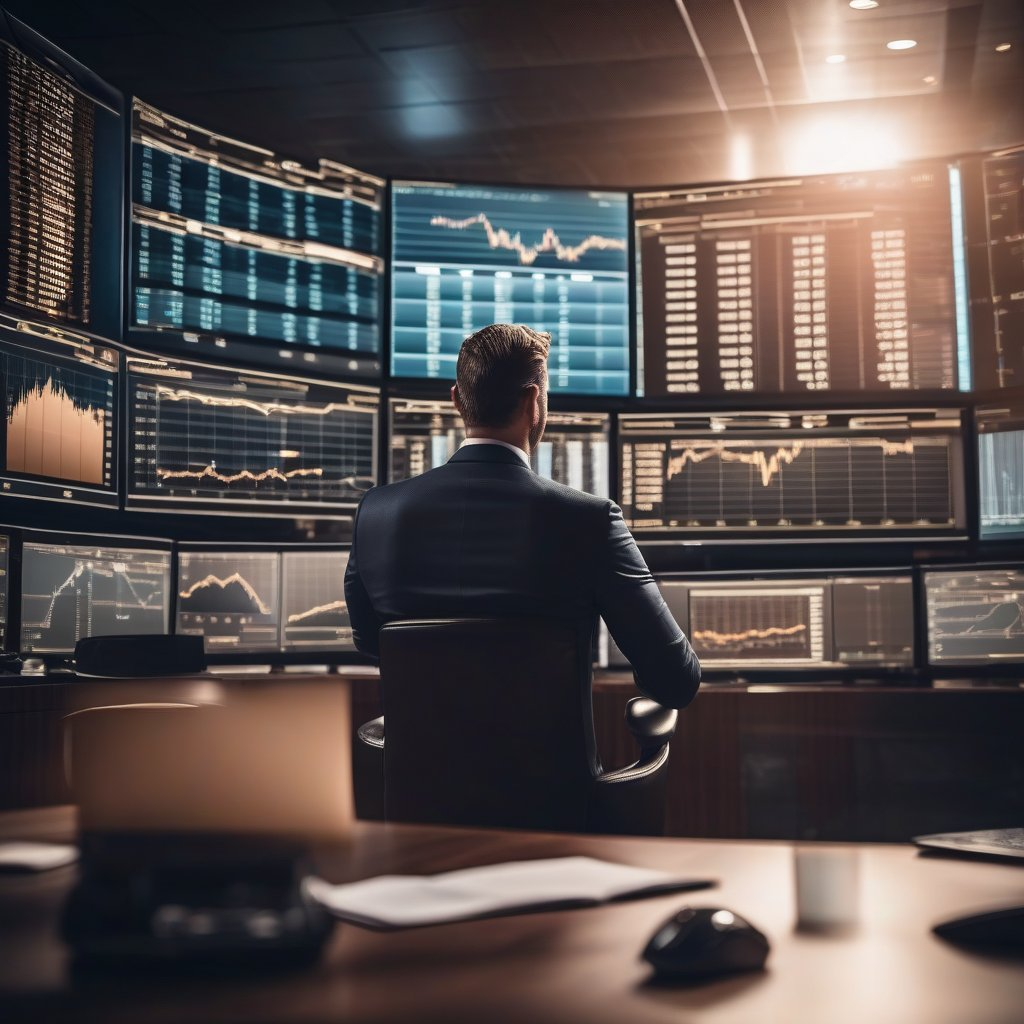
\includegraphics[width=0.45\textwidth,height=\textheight]{images/aitrader.jpg}
\end{center}

\textbf{Steps to take:}

\begin{enumerate}
\def\labelenumi{\arabic{enumi}.}
\item
  \textbf{Data Collection:} You gather historical price data for the
  stock of interest, including daily opening, closing, high, and low
  prices. Additionally, you collect relevant market data such as trading
  volume, volatility, and any external factors that may influence the
  stock's performance.
\item
  \textbf{Feature Engineering:} Employing your knowledge of technical
  analysis, you create additional features derived from the raw price
  data. These could include moving averages, Relative Strength Index
  (RSI), Bollinger Bands, and other indicators commonly used in
  financial analysis.
\item
  \textbf{Machine Learning Model Selection:} You choose a machine
  learning model suited for time-series forecasting, such as a recurrent
  neural network (RNN), long short-term memory network (LSTM), or a
  gradient boosting algorithm. The model should be capable of capturing
  patterns and trends in sequential data.
\item
  \textbf{Training the Model:} Using a subset of your historical data,
  you train the machine learning model to learn patterns and
  relationships between various features and the target variables (next
  day's high and low prices). You fine-tune the model parameters to
  enhance its predictive accuracy.
\item
  \textbf{Validation and Testing:} You validate the model's performance
  on a separate dataset that it hasn't seen during training. This step
  helps ensure that the model generalizes well to new, unseen data. Once
  satisfied with the validation results, you proceed to test the model
  on an out-of-sample dataset.
\item
  \textbf{Implementation and Integration:} Once the model demonstrates
  robust predictive capabilities, you integrate it into your trading
  strategy. Before each trading day, you input the latest available data
  to generate predictions for the next day's high and low prices.
\item
  \textbf{Decision Support:} The predicted high and low prices serve as
  valuable inputs in your decision-making process. You use this
  information to set limit orders, stop-loss levels, and identify
  potential entry and exit points based on your risk tolerance and
  trading strategy.
\item
  \textbf{Continuous Monitoring and Iteration:} Recognizing the dynamic
  nature of financial markets, you continuously monitor the model's
  performance and iterate on its architecture or features as needed.
  This adaptive approach ensures that your predictive model remains
  relevant in changing market conditions.
\end{enumerate}

\textbf{Outcomes:}

By incorporating predictive analytics into your trading strategy, you
gain a competitive advantage. The ability to forecast the next day's
high and low prices empowers you to make more informed and strategic
trading decisions. This approach allows you to optimize your risk-reward
ratio, adapt to market trends, and potentially enhance your overall
trading performance.

It's important to note that while predictive models can offer valuable
insights, no forecasting method is foolproof. Risk management and a
thorough understanding of market dynamics remain crucial aspects of
successful trading.

In this scenario, you will use PyTorch to build a deep learning model
that can predict the next day's high and low prices of a particular
asset. you will start by collecting historical data on the asset's price
movements, as well as any relevant external factors that could impact
its price. you will then preprocess this data and split it into
training, validation, and test sets.

Next, you will design and train a PyTorch model using the training set.
you will use a combination of convolutional and recurrent neural
networks to capture the complex patterns and trends in the data. you
will also use techniques such as batch normalization and regularization
to prevent overfitting and improve the model's generalization
performance.

Once the model is trained, you will evaluate its performance on the
validation set. you will use metrics such as mean absolute error and
mean squared error to assess the model's accuracy and precision. If the
model performs well on the validation set, you will use it to make
predictions on the test set.

The next step will be to use the model to predict the next day's high
and low prices of the asset. you will feed the model with the current
day's price data and any other relevant information, and it will output
the predicted high and low prices for the next day. you will then
compare these predictions with the actual prices to assess the model's
accuracy.

Finally, you will use the model's predictions to inform your trading
decisions. By knowing the predicted high and low prices of the asset,
you can better anticipate its future price movements and make more
informed trading decisions.

This could give you a competitive advantage in the market, allowing you
to make more profitable trades and outperform your competitors.
Throughout this process, you will also provide detailed mathematical
proofs for each project, using PyTorch's built-in tensor operations and
mathematical functions. This will allow you to demonstrate the
mathematical underpinnings of the model and provide a deeper
understanding of how it works. In conclusion, by using PyTorch to
predict the next day's high and low prices of an asset, you can gain a
competitive advantage in the financial markets. By combining machine
learning algorithms with mathematical proofs, you can build a robust and
accurate model that can help you make more informed trading decisions
and achieve better results.

As an individual trader aiming to gain a competitive advantage in the
financial markets, let's explore a scenario where you employ predictive
analytics to forecast the next day's high and low prices. In this
example, you'll leverage historical price data, technical indicators,
and machine learning algorithms to inform your trading decisions.

\chapter{Data Collection}\label{data-collection}

\section{Python Virtual Environment}\label{python-virtual-environment}

A virtual environment in Python is a self-contained directory that
encapsulates a specific Python interpreter along with its own set of
libraries and dependencies. It allows you to create isolated
environments for different Python projects, each with its own set of
packages, without interfering with the system-wide Python installation.

Here are some key concepts related to virtual environments in Python:

\begin{enumerate}
\def\labelenumi{\arabic{enumi}.}
\tightlist
\item
  \textbf{Isolation:}

  \begin{itemize}
  \tightlist
  \item
    A virtual environment provides a segregated space where you can
    install Python packages without affecting the global Python
    environment. This isolation is crucial when working on multiple
    projects that might require different versions of libraries or have
    conflicting dependencies.
  \end{itemize}
\item
  \textbf{Package Management:}

  \begin{itemize}
  \tightlist
  \item
    With a virtual environment, you can install, upgrade, and remove
    Python packages using tools like \texttt{pip} without affecting the
    rest of your system. This ensures that each project has its own set
    of dependencies.
  \end{itemize}
\item
  \textbf{Version Control:}

  \begin{itemize}
  \tightlist
  \item
    Virtual environments help manage Python interpreter versions. You
    can create a virtual environment with a specific version of Python,
    ensuring consistency across different projects. This is particularly
    useful when transitioning between Python 2 and Python 3 or when
    working with different Python versions for compatibility reasons.
  \end{itemize}
\item
  \textbf{Dependency Management:}

  \begin{itemize}
  \tightlist
  \item
    Virtual environments allow you to specify and manage dependencies
    for each project. You can create a \texttt{requirements.txt} file
    listing all the dependencies and their versions, making it easy for
    others to recreate the same environment.
  \end{itemize}
\item
  \textbf{Activation and Deactivation:}

  \begin{itemize}
  \tightlist
  \item
    Activating a virtual environment modifies the system's \texttt{PATH}
    variable to prioritize the virtual environment's binaries. This
    means that when you run Python or use \texttt{pip}, it refers to the
    versions within the virtual environment. Once your work in the
    virtual environment is done, you can deactivate it to return to the
    global Python environment.
  \end{itemize}
\item
  \textbf{Cleaner Project Directories:}

  \begin{itemize}
  \tightlist
  \item
    Virtual environments keep project directories clean by isolating
    project-specific dependencies. This makes it easier to share
    projects with others and avoids conflicts with system-wide packages.
  \end{itemize}
\item
  \textbf{Compatibility:}

  \begin{itemize}
  \tightlist
  \item
    Virtual environments are compatible across operating systems. You
    can create a virtual environment on one machine, and someone else
    can recreate the same environment on a different machine by using
    the same configuration files (e.g., \texttt{requirements.txt}).
  \end{itemize}
\item
  \textbf{Built-in Modules:}

  \begin{itemize}
  \tightlist
  \item
    Python comes with a built-in module called \texttt{venv} (since
    Python 3.3) for creating virtual environments. Additionally, popular
    third-party tools like \texttt{virtualenv} and \texttt{conda} can
    also be used to create virtual environments.
  \end{itemize}
\end{enumerate}

To summarize, virtual environments in Python are a valuable tool for
managing project-specific dependencies, ensuring version consistency,
and maintaining a clean and organized development environment. They
contribute to better project portability, reproducibility, and efficient
collaboration among developers.

Creating Anaconda environments and virtual environments in Python can be
a straightforward process. Below are the steps for both Windows and
Linux:

\subsection{Creating an Anaconda
Environment:}\label{creating-an-anaconda-environment}

\subsubsection{For Windows:}\label{for-windows}

\begin{enumerate}
\def\labelenumi{\arabic{enumi}.}
\item
  \textbf{Download and Install Anaconda:}

  \begin{itemize}
  \tightlist
  \item
    Download the Anaconda distribution for Windows from the
    \href{https://www.anaconda.com/products/distribution}{official
    Anaconda website}.
  \item
    Run the installer and follow the installation instructions.
  \end{itemize}
\item
  \textbf{Open Anaconda Navigator:}

  \begin{itemize}
  \tightlist
  \item
    Once installed, open the Anaconda Navigator.
  \end{itemize}
\item
  \textbf{Create a New Environment:}

  \begin{itemize}
  \tightlist
  \item
    Click on the ``Environments'' tab.
  \item
    Click the ``Create'' button.
  \item
    Enter a name for your new environment, select Python version, and
    choose the packages you need.
  \item
    Click ``Create'' to create the environment.
  \end{itemize}
\item
  \textbf{Activate the Environment:}

  \begin{itemize}
  \tightlist
  \item
    To activate the environment, open the ``Home'' tab.
  \item
    From the Applications on the left, select ``Home'' and then choose
    your environment from the drop-down list.
  \item
    Click on ``Home'' again, and you should see your environment name in
    the right pane.
  \item
    Click ``Install'' to install packages in the selected environment.
  \end{itemize}
\item
  To create a new environment using Conda, you can use the
  \texttt{conda\ create} command. Below are the basic steps:

  \subsection{Create a new Conda
  environment:}\label{create-a-new-conda-environment}

  \begin{enumerate}
  \def\labelenumii{\arabic{enumii}.}
  \item
    \textbf{Open a terminal or command prompt:}

    \begin{itemize}
    \tightlist
    \item
      On Windows, you can use the Anaconda Prompt or any command prompt.
    \item
      On Linux or macOS, you can use a terminal.
    \end{itemize}
  \item
    \textbf{Run the following command:}

\begin{Shaded}
\begin{Highlighting}[]
\ExtensionTok{conda}\NormalTok{ create }\AttributeTok{{-}{-}name}\NormalTok{ your\_environment\_name python=3.x}
\end{Highlighting}
\end{Shaded}

    Replace \texttt{your\_environment\_name} with the desired name for
    your new environment, and \texttt{3.x} with the desired Python
    version (e.g., \texttt{3.8}).

    For example, to create an environment named ``myenv'' with Python
    3.8, you would run:

\begin{Shaded}
\begin{Highlighting}[]
\ExtensionTok{conda}\NormalTok{ create }\AttributeTok{{-}{-}name}\NormalTok{ myenv python=3.8}
\end{Highlighting}
\end{Shaded}
  \item
    \textbf{Activate the new environment:}

    \begin{itemize}
    \item
      On Windows:

\begin{Shaded}
\begin{Highlighting}[]
\ExtensionTok{conda}\NormalTok{ activate your\_environment\_name}
\end{Highlighting}
\end{Shaded}
    \item
      On Linux or macOS:

\begin{Shaded}
\begin{Highlighting}[]
\BuiltInTok{source}\NormalTok{ activate your\_environment\_name}
\end{Highlighting}
\end{Shaded}

      Replace \texttt{your\_environment\_name} with the name you
      provided earlier.
    \end{itemize}

    After activation, your command prompt or terminal should indicate
    that you are now working in the new environment.
  \item
    \textbf{Install additional packages (optional):}

    \begin{itemize}
    \item
      You can install additional packages in your new environment using
      \texttt{conda\ install} or \texttt{pip\ install} as needed. For
      example:

\begin{Shaded}
\begin{Highlighting}[]
\ExtensionTok{conda}\NormalTok{ install numpy pandas}
\end{Highlighting}
\end{Shaded}
    \end{itemize}
  \item
    \textbf{Deactivate the environment (when done):}

    \begin{itemize}
    \item
      When you're finished working in the environment, you can
      deactivate it using the following command:

\begin{Shaded}
\begin{Highlighting}[]
\ExtensionTok{conda}\NormalTok{ deactivate}
\end{Highlighting}
\end{Shaded}

      This will return you to the base (root) environment.
    \end{itemize}
  \end{enumerate}

  \subsection{Note:}\label{note}

  \begin{itemize}
  \tightlist
  \item
    It's a good practice to include the Python version when creating a
    new environment to ensure compatibility.
  \item
    You can customize the environment further by installing specific
    versions of packages or specifying additional packages during the
    creation process.
  \item
    Remember to activate the environment whenever you want to work
    within it, and deactivate it when you're finished.
  \end{itemize}

  By following these steps, you can create and manage Conda environments
  for your Python projects.
\end{enumerate}

\subsubsection{For Linux:}\label{for-linux}

\begin{enumerate}
\def\labelenumi{\arabic{enumi}.}
\tightlist
\item
  \textbf{Download and Install Anaconda:}

  \begin{itemize}
  \tightlist
  \item
    Download the Anaconda distribution for Linux from the
    \href{https://www.anaconda.com/products/distribution}{official
    Anaconda website}.
  \item
    Open a terminal in the directory where the installer was downloaded.
  \item
    Run the following command to install Anaconda:
    \texttt{bash\ Anaconda3-\textless{}version\textgreater{}-Linux-x86\_64.sh}
  \item
    Follow the on-screen instructions to complete the installation.
  \end{itemize}
\item
  \textbf{Open Anaconda Navigator:}

  \begin{itemize}
  \tightlist
  \item
    Once installed, open a terminal and run \texttt{anaconda-navigator}.
  \end{itemize}
\item
  \textbf{Create a New Environment:}

  \begin{itemize}
  \tightlist
  \item
    In Anaconda Navigator, go to the ``Environments'' tab.
  \item
    Click the ``Create'' button.
  \item
    Enter a name for your new environment, select Python version, and
    choose the packages you need.
  \item
    Click ``Create'' to create the environment.
  \end{itemize}
\item
  \textbf{Activate the Environment:}

  \begin{itemize}
  \tightlist
  \item
    To activate the environment, open a terminal and run:
    \texttt{conda\ activate\ your\_environment\_name}
  \item
    Replace \texttt{your\_environment\_name} with the actual name of
    your environment.
  \end{itemize}
\end{enumerate}

\subsection{Creating a Virtual
Environment:}\label{creating-a-virtual-environment}

\subsubsection{For Windows:}\label{for-windows-1}

\begin{enumerate}
\def\labelenumi{\arabic{enumi}.}
\tightlist
\item
  \textbf{Open a Command Prompt:}

  \begin{itemize}
  \tightlist
  \item
    Open the command prompt.
  \end{itemize}
\item
  \textbf{Install \texttt{virtualenv}:}

  \begin{itemize}
  \tightlist
  \item
    Run the following command to install \texttt{virtualenv}:
    \texttt{pip\ install\ virtualenv}
  \end{itemize}
\item
  \textbf{Create a Virtual Environment:}

  \begin{itemize}
  \tightlist
  \item
    Navigate to the directory where you want to create the virtual
    environment.
  \item
    Run the following command:
    \texttt{python\ -m\ venv\ your\_virtual\_environment}
  \item
    Replace \texttt{your\_virtual\_environment} with the desired name
    for your virtual environment.
  \end{itemize}
\item
  \textbf{Activate the Virtual Environment:}

  \begin{itemize}
  \tightlist
  \item
    Navigate to the virtual environment's directory.
  \item
    Run:
    \texttt{.\textbackslash{}your\_virtual\_environment\textbackslash{}Scripts\textbackslash{}activate}
  \item
    You should see the virtual environment name in the command prompt.
  \end{itemize}
\end{enumerate}

\subsubsection{For Linux:}\label{for-linux-1}

\begin{enumerate}
\def\labelenumi{\arabic{enumi}.}
\tightlist
\item
  \textbf{Open a Terminal:}

  \begin{itemize}
  \tightlist
  \item
    Open a terminal.
  \end{itemize}
\item
  \textbf{Install \texttt{virtualenv}:}

  \begin{itemize}
  \tightlist
  \item
    Run the following command to install \texttt{virtualenv}:
    \texttt{pip\ install\ virtualenv}
  \end{itemize}
\item
  \textbf{Create a Virtual Environment:}

  \begin{itemize}
  \tightlist
  \item
    Navigate to the directory where you want to create the virtual
    environment.
  \item
    Run the following command:
    \texttt{python\ -m\ venv\ your\_virtual\_environment}
  \item
    Replace \texttt{your\_virtual\_environment} with the desired name
    for your virtual environment.
  \end{itemize}
\item
  \textbf{Activate the Virtual Environment:}

  \begin{itemize}
  \tightlist
  \item
    Navigate to the virtual environment's directory.
  \item
    Run: \texttt{source\ your\_virtual\_environment/bin/activate}
  \item
    You should see the virtual environment name in the terminal.
  \end{itemize}
\end{enumerate}

These steps should help you create Anaconda environments and virtual
environments on both Windows and Linux systems. Adjust the environment
names and versions as needed.

So lets create and activate an anaconda environment for our project.

\begin{Shaded}
\begin{Highlighting}[]

\ExtensionTok{conda}\NormalTok{ create }\AttributeTok{{-}{-}name}\NormalTok{ dppa }\AttributeTok{{-}y}
\ExtensionTok{conda}\NormalTok{ activate dppa}
\end{Highlighting}
\end{Shaded}

\begin{tcolorbox}[enhanced jigsaw, bottomtitle=1mm, bottomrule=.15mm, colbacktitle=quarto-callout-note-color!10!white, breakable, titlerule=0mm, title=\textcolor{quarto-callout-note-color}{\faInfo}\hspace{0.5em}{Note}, left=2mm, colframe=quarto-callout-note-color-frame, arc=.35mm, toprule=.15mm, coltitle=black, colback=white, opacityback=0, toptitle=1mm, rightrule=.15mm, leftrule=.75mm, opacitybacktitle=0.6]

The given Bash command (\textbf{bash\_conda\_create?}) is a Conda
command used to create a new Conda environment. Let's break down the
components of the command:

\begin{itemize}
\item
  \texttt{conda\ create}: This part of the command instructs Conda to
  create a new environment.
\item
  \texttt{-\/-name\ dppa}: This option specifies the name of the new
  environment. In this case, the environment is named ``dppa.'' You can
  replace ``dppa'' with any desired name for your environment.
\item
  \texttt{-y}: This option stands for ``yes'' and is used to
  automatically confirm and proceed with the installation without
  prompting the user for confirmation. Adding \texttt{-y} is useful,
  especially when you want to automate environment creation in scripts
  or ensure a smooth, non-interactive installation.
\end{itemize}

Putting it all together, the command
\texttt{conda\ create\ -\/-name\ dppa\ -y} creates a new Conda
environment named ``dppa'' without asking for user confirmation during
the process. This environment can later be activated and used for
specific Python projects, allowing for isolation and management of
dependencies.

\end{tcolorbox}

\section{Data Collection}\label{data-collection-1}

We are going to use \textbf{\texttt{yfinance}} to fetch historical data.
\textbf{\texttt{yfinance}} is a Python library that provides a simple
and convenient way to access financial data from Yahoo Finance. Yahoo
Finance is a popular platform that offers a wide range of financial
information, including historical stock prices, current market data,
company information, and more. Here are the main functionalities and
features of the \textbf{\texttt{yfinance}} library:

\begin{enumerate}
\def\labelenumi{\arabic{enumi}.}
\item
  \textbf{Historical Data Retrieval:}

  \begin{itemize}
  \tightlist
  \item
    \textbf{\texttt{yfinance}} allows users to download historical stock
    price data for a specific ticker symbol over a specified time
    period. This data includes daily Open, High, Low, Close prices, and
    trading volume.
  \end{itemize}
\item
  \textbf{Current Market Data:}

  \begin{itemize}
  \tightlist
  \item
    Users can retrieve real-time market data, including the latest stock
    price, bid and ask prices, trading volume, and more.
  \end{itemize}
\item
  \textbf{Dividend and Split Information:}

  \begin{itemize}
  \tightlist
  \item
    The library provides access to information about dividends and stock
    splits for a given ticker symbol.
  \end{itemize}
\item
  \textbf{Financial Statements and Company Information:}

  \begin{itemize}
  \tightlist
  \item
    \textbf{\texttt{yfinance}} enables users to fetch financial
    statements, such as income statements, balance sheets, and cash flow
    statements. It also provides general information about a company,
    including its name, sector, and industry.
  \end{itemize}
\item
  \textbf{Option and Warrant Data:}

  \begin{itemize}
  \tightlist
  \item
    Users can obtain option and warrant data, including details on
    options chains and expiration dates.
  \end{itemize}
\item
  \textbf{Support for Multiple Ticker Symbols:}

  \begin{itemize}
  \tightlist
  \item
    The library supports the retrieval of data for multiple ticker
    symbols in a single call, allowing for efficient data retrieval for
    a portfolio of stocks.
  \end{itemize}
\item
  \textbf{Customizable Date Ranges:}

  \begin{itemize}
  \tightlist
  \item
    Users can specify custom start and end dates to retrieve historical
    data for a specific time period.
  \end{itemize}
\end{enumerate}

\begin{Shaded}
\begin{Highlighting}[]
\ImportTok{import}\NormalTok{ yfinance }\ImportTok{as}\NormalTok{ yf}
\ImportTok{import}\NormalTok{ pandas }\ImportTok{as}\NormalTok{ pd}
\ImportTok{import}\NormalTok{ seaborn }\ImportTok{as}\NormalTok{ sns}
\ImportTok{import}\NormalTok{ matplotlib.pyplot }\ImportTok{as}\NormalTok{ plt}

\KeywordTok{def}\NormalTok{ fetch\_stock\_data(ticker, start\_date, end\_date):}
    \CommentTok{"""}
\CommentTok{    Fetch historical stock data for a given ticker symbol.}

\CommentTok{    Parameters:}
\CommentTok{    {-} ticker: Stock ticker symbol (e.g., AAPL for Apple Inc.).}
\CommentTok{    {-} start\_date: Start date for historical data in \textquotesingle{}YYYY{-}MM{-}DD\textquotesingle{} format.}
\CommentTok{    {-} end\_date: End date for historical data in \textquotesingle{}YYYY{-}MM{-}DD\textquotesingle{} format.}

\CommentTok{    Returns:}
\CommentTok{    {-} A DataFrame containing historical stock data.}
\CommentTok{    """}
\NormalTok{    stock\_data }\OperatorTok{=}\NormalTok{ yf.download(ticker, start}\OperatorTok{=}\NormalTok{start\_date, end}\OperatorTok{=}\NormalTok{end\_date, progress}\OperatorTok{=}\VariableTok{False}\NormalTok{)}
    \ControlFlowTok{return}\NormalTok{ stock\_data}

\KeywordTok{def}\NormalTok{ calculate\_metrics(historical\_data):}
    \CommentTok{"""}
\CommentTok{    Calculate Volatility, Volume, and Performance metrics.}

\CommentTok{    Parameters:}
\CommentTok{    {-} historical\_data: DataFrame containing historical stock data.}

\CommentTok{    Returns:}
\CommentTok{    {-} DataFrame with added columns for Volatility, Volume, and Performance.}
\CommentTok{    """}
    \CommentTok{\# Calculate Volatility}
\NormalTok{    historical\_data[}\StringTok{\textquotesingle{}Volatility\textquotesingle{}}\NormalTok{] }\OperatorTok{=}\NormalTok{ historical\_data[}\StringTok{\textquotesingle{}Close\textquotesingle{}}\NormalTok{].pct\_change().rolling(window}\OperatorTok{=}\DecValTok{252}\NormalTok{).std() }\OperatorTok{*}\NormalTok{ (}\DecValTok{252}\OperatorTok{**}\FloatTok{0.5}\NormalTok{)}
    
    \CommentTok{\# Calculate Volume}
\NormalTok{    historical\_data[}\StringTok{\textquotesingle{}Volume\textquotesingle{}}\NormalTok{] }\OperatorTok{=}\NormalTok{ historical\_data[}\StringTok{\textquotesingle{}Volume\textquotesingle{}}\NormalTok{].rolling(window}\OperatorTok{=}\DecValTok{252}\NormalTok{).mean()}
    
    \CommentTok{\# Calculate Performance}
\NormalTok{    historical\_data[}\StringTok{\textquotesingle{}Performance\textquotesingle{}}\NormalTok{] }\OperatorTok{=}\NormalTok{ historical\_data[}\StringTok{\textquotesingle{}Close\textquotesingle{}}\NormalTok{].pct\_change() }\OperatorTok{*} \DecValTok{100}

    \ControlFlowTok{return}\NormalTok{ historical\_data}

\KeywordTok{def}\NormalTok{ plot\_metrics(historical\_data):}
    \CommentTok{"""}
\CommentTok{    Plot Volatility, Volume, and Performance using seaborn.}

\CommentTok{    Parameters:}
\CommentTok{    {-} historical\_data: DataFrame containing historical stock data with added metrics.}
\CommentTok{    """}
\NormalTok{    sns.}\BuiltInTok{set}\NormalTok{(style}\OperatorTok{=}\StringTok{"whitegrid"}\NormalTok{)}
\NormalTok{    plt.figure(figsize}\OperatorTok{=}\NormalTok{(}\DecValTok{8}\NormalTok{, }\DecValTok{8}\NormalTok{))}

    \CommentTok{\# Plot Volatility}
\NormalTok{    plt.subplot(}\DecValTok{3}\NormalTok{, }\DecValTok{1}\NormalTok{, }\DecValTok{1}\NormalTok{)}
\NormalTok{    sns.lineplot(data}\OperatorTok{=}\NormalTok{historical\_data[}\StringTok{\textquotesingle{}Volatility\textquotesingle{}}\NormalTok{], color}\OperatorTok{=}\StringTok{\textquotesingle{}blue\textquotesingle{}}\NormalTok{)}
\NormalTok{    plt.title(}\StringTok{\textquotesingle{}Volatility\textquotesingle{}}\NormalTok{)}

    \CommentTok{\# Plot Volume}
\NormalTok{    plt.subplot(}\DecValTok{3}\NormalTok{, }\DecValTok{1}\NormalTok{, }\DecValTok{2}\NormalTok{)}
\NormalTok{    sns.lineplot(data}\OperatorTok{=}\NormalTok{historical\_data[}\StringTok{\textquotesingle{}Volume\textquotesingle{}}\NormalTok{], color}\OperatorTok{=}\StringTok{\textquotesingle{}orange\textquotesingle{}}\NormalTok{)}
\NormalTok{    plt.title(}\StringTok{\textquotesingle{}Volume\textquotesingle{}}\NormalTok{)}

    \CommentTok{\# Plot Performance}
\NormalTok{    plt.subplot(}\DecValTok{3}\NormalTok{, }\DecValTok{1}\NormalTok{, }\DecValTok{3}\NormalTok{)}
\NormalTok{    sns.lineplot(data}\OperatorTok{=}\NormalTok{historical\_data[}\StringTok{\textquotesingle{}Performance\textquotesingle{}}\NormalTok{], color}\OperatorTok{=}\StringTok{\textquotesingle{}green\textquotesingle{}}\NormalTok{)}
\NormalTok{    plt.title(}\StringTok{\textquotesingle{}Performance\textquotesingle{}}\NormalTok{)}

\NormalTok{    plt.tight\_layout()}
\NormalTok{    plt.show()}

\CommentTok{\# Example usage:}
\NormalTok{ticker\_symbol }\OperatorTok{=} \StringTok{"AAPL"}  \CommentTok{\# Replace with the desired stock symbol}
\NormalTok{start\_date }\OperatorTok{=} \StringTok{"2021{-}01{-}01"}
\NormalTok{end\_date }\OperatorTok{=} \StringTok{"2023{-}12{-}12"}

\NormalTok{historical\_data }\OperatorTok{=}\NormalTok{ fetch\_stock\_data(ticker\_symbol, start\_date, end\_date)}
\NormalTok{historical\_data\_with\_metrics }\OperatorTok{=}\NormalTok{ calculate\_metrics(historical\_data)}
\NormalTok{plot\_metrics(historical\_data\_with\_metrics)}
\end{Highlighting}
\end{Shaded}

\begin{figure}[H]

\centering{

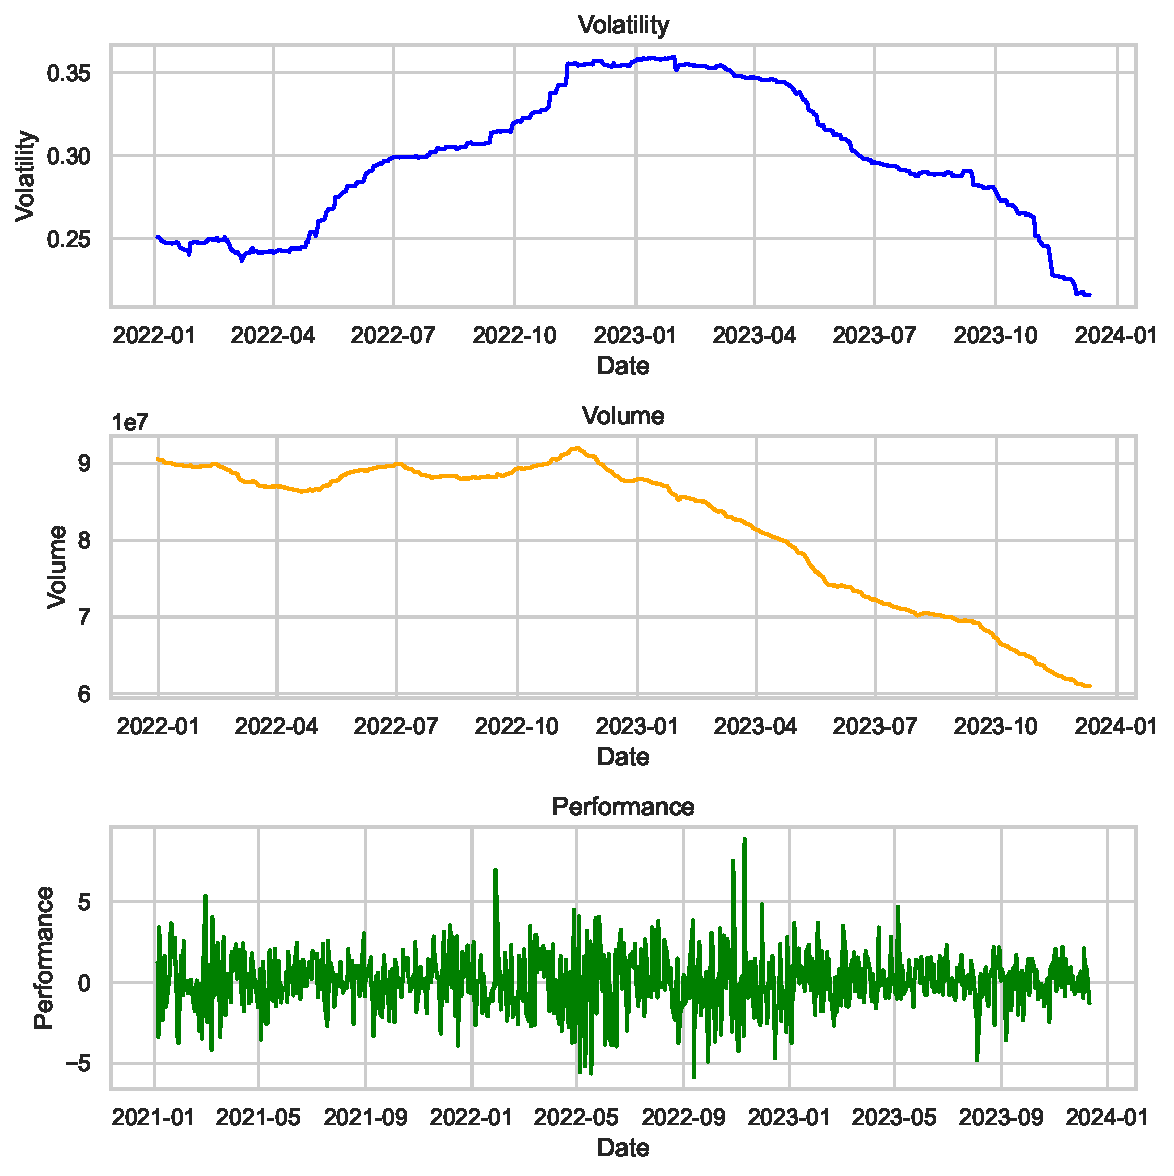
\includegraphics{trading/Data Collection_files/figure-pdf/fig-plot-output-1.pdf}

}

\caption{\label{fig-plot}Plot Volatility, Volume, and Performance}

\end{figure}%

This code provides a visual representation of how these financial
indicators change over time as shown in Figure~\ref{fig-plot}.
Volatility is shown in blue, Volume in orange, and Performance in green.
The \texttt{rolling} function is used to calculate these metrics over a
specified window, providing a smoothed representation of their trends.
The resulting plot helps in understanding the historical behavior of
these indicators for the given stock. In the example, the
\texttt{yfinance} library is used to fetch historical stock data. You
can install it using the command \texttt{pip\ install\ yfinance}. Adjust
the \texttt{ticker\_symbol}, \texttt{start\_date}, and
\texttt{end\_date} variables according to your requirements.

Please note that using this approach, you can gather basic historical
price data. For more extensive financial data and external factors that
may influence stock performance, you may need to integrate other data
sources or APIs into your code.

\begin{enumerate}
\def\labelenumi{\arabic{enumi}.}
\item
  \textbf{Calculate Volatility:}

  \begin{itemize}
  \item
    Volatility is often measured as the standard deviation of the daily
    returns. In finance, it's a common metric used to assess the
    variability of a stock's price. The formula for calculating
    volatility is:
    \(\text{Volatility} = \sqrt{\frac{\sum_{i=1}^{N}(R_i - \bar{R})^2}{N}}\)
    where \(R_i\) is the daily return, \(\bar{R}\) is the mean of daily
    returns, and \(N\) is the number of days (in this case, the rolling
    window of 252 days).
  \item
    Code for calculating volatility:

\begin{Shaded}
\begin{Highlighting}[]
\NormalTok{historical\_data[}\StringTok{\textquotesingle{}Volatility\textquotesingle{}}\NormalTok{] }\OperatorTok{=}\NormalTok{ historical\_data[}\StringTok{\textquotesingle{}Close\textquotesingle{}}\NormalTok{].rolling(window}\OperatorTok{=}\DecValTok{252}\NormalTok{).std() }
\end{Highlighting}
\end{Shaded}
  \end{itemize}
\item
  \textbf{Calculate Volume:}

  \begin{itemize}
  \item
    Volume is often used as a measure of market activity. It represents
    the total number of shares traded in a day. In this case, the
    rolling mean over a window of 252 days is calculated to smooth out
    short-term fluctuations. The formula is straightforward:
    \(\text{Volume} = \frac{\sum_{i=1}^{N}\text{Volume}_i}{N}\)
  \item
    Code for calculating volume:

\begin{Shaded}
\begin{Highlighting}[]
\NormalTok{historical\_data[}\StringTok{\textquotesingle{}Volume\textquotesingle{}}\NormalTok{] }\OperatorTok{=}\NormalTok{ historical\_data[}\StringTok{\textquotesingle{}Volume\textquotesingle{}}\NormalTok{].rolling(window}\OperatorTok{=}\DecValTok{252}\NormalTok{).mean()}
\end{Highlighting}
\end{Shaded}
  \end{itemize}
\item
  \textbf{Calculate Performance:}

  \begin{itemize}
  \item
    Performance is typically measured as the percentage change in the
    closing price from one day to the next. This helps assess the daily
    returns of the stock. The formula is:
    \[\text{Performance}_i = \frac{\text{Close}_{i} - \text{Close}_{i-1}}{\text{Close}_{i-1}}\times 100\]
    This represents the percentage change in the closing price from day
    (i-1) to day (i).
  \item
    Code for calculating performance:

\begin{Shaded}
\begin{Highlighting}[]
\NormalTok{historical\_data[}\StringTok{\textquotesingle{}Performance\textquotesingle{}}\NormalTok{] }\OperatorTok{=}\NormalTok{ historical\_data[}\StringTok{\textquotesingle{}Close\textquotesingle{}}\NormalTok{].pct\_change()}
\end{Highlighting}
\end{Shaded}
  \end{itemize}
\item
  \textbf{Plotting:}

  \begin{itemize}
  \item
    Finally, the three indicators - Volatility, Volume, and Performance
    - are plotted using \texttt{matplotlib}. The different colors and
    labels are added to differentiate between the lines in the plot.

\phantomsection\label{annotated-cell-13}%
\begin{Shaded}
\begin{Highlighting}[]
\NormalTok{    sns.}\BuiltInTok{set}\NormalTok{(style}\OperatorTok{=}\StringTok{"whitegrid"}\NormalTok{)}
\NormalTok{    plt.figure(figsize}\OperatorTok{=}\NormalTok{(}\DecValTok{12}\NormalTok{, }\DecValTok{8}\NormalTok{))}

    \CommentTok{\# Plot Volatility}
\NormalTok{    plt.subplot(}\DecValTok{3}\NormalTok{, }\DecValTok{1}\NormalTok{, }\DecValTok{1}\NormalTok{) }\hspace*{\fill}\NormalTok{\circled{1}}
\NormalTok{    sns.lineplot(data}\OperatorTok{=}\NormalTok{historical\_data[}\StringTok{\textquotesingle{}Volatility\textquotesingle{}}\NormalTok{], color}\OperatorTok{=}\StringTok{\textquotesingle{}blue\textquotesingle{}}\NormalTok{) }
\NormalTok{    plt.title(}\StringTok{\textquotesingle{}Volatility\textquotesingle{}}\NormalTok{) }

    \CommentTok{\# Plot Volume}
\NormalTok{    plt.subplot(}\DecValTok{3}\NormalTok{, }\DecValTok{1}\NormalTok{, }\DecValTok{2}\NormalTok{) }\hspace*{\fill}\NormalTok{\circled{2}}
\NormalTok{    sns.lineplot(data}\OperatorTok{=}\NormalTok{historical\_data[}\StringTok{\textquotesingle{}Volume\textquotesingle{}}\NormalTok{], color}\OperatorTok{=}\StringTok{\textquotesingle{}orange\textquotesingle{}}\NormalTok{) }
\NormalTok{    plt.title(}\StringTok{\textquotesingle{}Volume\textquotesingle{}}\NormalTok{)}

    \CommentTok{\# Plot Performance}
\NormalTok{    plt.subplot(}\DecValTok{3}\NormalTok{, }\DecValTok{1}\NormalTok{, }\DecValTok{3}\NormalTok{) }\hspace*{\fill}\NormalTok{\circled{3}}
\NormalTok{    sns.lineplot(data}\OperatorTok{=}\NormalTok{historical\_data[}\StringTok{\textquotesingle{}Performance\textquotesingle{}}\NormalTok{], color}\OperatorTok{=}\StringTok{\textquotesingle{}green\textquotesingle{}}\NormalTok{) }
\NormalTok{    plt.title(}\StringTok{\textquotesingle{}Performance\textquotesingle{}}\NormalTok{) }

\NormalTok{    plt.tight\_layout()}
\NormalTok{    plt.show()}
\end{Highlighting}
\end{Shaded}
  \end{itemize}
\end{enumerate}

\subsection{Data Reprocessing}\label{data-reprocessing}

Data preprocessing is a crucial step in preparing financial data for use
in a trading algorithm. The goal is to clean, transform, and structure
the data to make it suitable for analysis and modeling. Below are common
steps involved in data preprocessing for a trading algorithm using
\texttt{yfinance} data:

\subsection{\texorpdfstring{1. \textbf{Data
Retrieval:}}{1. Data Retrieval:}}\label{data-retrieval}

\begin{itemize}
\item
  Use \texttt{yfinance} to download historical stock price data for the
  desired ticker symbols and time period.

\begin{Shaded}
\begin{Highlighting}[]
\ImportTok{import}\NormalTok{ yfinance }\ImportTok{as}\NormalTok{ yf}

\CommentTok{\# Example: Fetch historical data for AAPL}
\NormalTok{historical\_data }\OperatorTok{=}\NormalTok{ yf.download(}\StringTok{"AAPL"}\NormalTok{, start}\OperatorTok{=}\StringTok{"2022{-}01{-}01"}\NormalTok{, end}\OperatorTok{=}\StringTok{"2023{-}01{-}01"}\NormalTok{, progress}\OperatorTok{=}\VariableTok{False}\NormalTok{)}
\end{Highlighting}
\end{Shaded}
\end{itemize}

\subsection{\texorpdfstring{2. \textbf{Handling Missing
Data:}}{2. Handling Missing Data:}}\label{handling-missing-data}

\begin{itemize}
\item
  Check for missing values in the dataset.
\item
  Decide on a strategy to handle missing data, such as interpolation,
  forward-fill, or backward-fill.

\begin{Shaded}
\begin{Highlighting}[]
\CommentTok{\# Check for missing values}
\NormalTok{missing\_values }\OperatorTok{=}\NormalTok{ historical\_data.isnull().}\BuiltInTok{sum}\NormalTok{()}

\CommentTok{\# Handle missing values (for example, forward{-}fill)}
\NormalTok{historical\_data }\OperatorTok{=}\NormalTok{ historical\_data.ffill()}
\end{Highlighting}
\end{Shaded}
\end{itemize}

\subsection{\texorpdfstring{3. \textbf{Feature
Engineering:}}{3. Feature Engineering:}}\label{feature-engineering}

\begin{itemize}
\item
  Create new features that might be useful for modeling, such as moving
  averages, technical indicators, or other relevant financial metrics.

\begin{Shaded}
\begin{Highlighting}[]
\CommentTok{\# Example: Calculate 10{-}day simple moving average}
\NormalTok{historical\_data[}\StringTok{\textquotesingle{}SMA\_10\textquotesingle{}}\NormalTok{] }\OperatorTok{=}\NormalTok{ historical\_data[}\StringTok{\textquotesingle{}Close\textquotesingle{}}\NormalTok{].rolling(window}\OperatorTok{=}\DecValTok{10}\NormalTok{).mean()}
\end{Highlighting}
\end{Shaded}
\end{itemize}

\subsection{\texorpdfstring{4.
\textbf{Normalization/Scaling:}}{4. Normalization/Scaling:}}\label{normalizationscaling}

\begin{itemize}
\item
  Normalize or scale numerical features to a common range, especially if
  using machine learning models sensitive to scale.

\begin{Shaded}
\begin{Highlighting}[]
\ImportTok{from}\NormalTok{ sklearn.preprocessing }\ImportTok{import}\NormalTok{ MinMaxScaler}

\CommentTok{\# Example: Normalize closing prices}
\NormalTok{scaler }\OperatorTok{=}\NormalTok{ MinMaxScaler()}
\NormalTok{historical\_data[}\StringTok{\textquotesingle{}Close\_Normalized\textquotesingle{}}\NormalTok{] }\OperatorTok{=}\NormalTok{ scaler.fit\_transform(historical\_data[}\StringTok{\textquotesingle{}Close\textquotesingle{}}\NormalTok{].values.reshape(}\OperatorTok{{-}}\DecValTok{1}\NormalTok{, }\DecValTok{1}\NormalTok{))}
\end{Highlighting}
\end{Shaded}
\end{itemize}

\subsection{\texorpdfstring{5. \textbf{Removing
Outliers:}}{5. Removing Outliers:}}\label{removing-outliers}

\begin{itemize}
\item
  Identify and handle outliers that might adversely affect model
  performance.

\begin{Shaded}
\begin{Highlighting}[]
\CommentTok{\# Example: Remove outliers using z{-}score}
\ImportTok{from}\NormalTok{ scipy.stats }\ImportTok{import}\NormalTok{ zscore}

\NormalTok{z\_scores }\OperatorTok{=}\NormalTok{ zscore(historical\_data[}\StringTok{\textquotesingle{}Close\textquotesingle{}}\NormalTok{])}
\NormalTok{historical\_data }\OperatorTok{=}\NormalTok{ historical\_data[(z\_scores }\OperatorTok{\textless{}} \DecValTok{3}\NormalTok{) }\OperatorTok{\&}\NormalTok{ (z\_scores }\OperatorTok{\textgreater{}} \OperatorTok{{-}}\DecValTok{3}\NormalTok{)]}
\end{Highlighting}
\end{Shaded}
\end{itemize}

\subsection{\texorpdfstring{6. \textbf{Time
Resampling:}}{6. Time Resampling:}}\label{time-resampling}

\begin{itemize}
\item
  Adjust the frequency of the data (e.g., daily to weekly) if needed.

\begin{Shaded}
\begin{Highlighting}[]
\CommentTok{\# Example: Resample data to weekly frequency}
\NormalTok{weekly\_data }\OperatorTok{=}\NormalTok{ historical\_data.resample(}\StringTok{\textquotesingle{}D\textquotesingle{}}\NormalTok{).last()}
\end{Highlighting}
\end{Shaded}
\end{itemize}

\subsection{\texorpdfstring{7.
\textbf{Labeling:}}{7. Labeling:}}\label{labeling}

\begin{itemize}
\item
  For supervised learning, create labels or target variables based on
  future price movements.

\begin{Shaded}
\begin{Highlighting}[]
\CommentTok{\# Example: Create binary labels for price increase (1) or decrease (0)}
\NormalTok{historical\_data[}\StringTok{\textquotesingle{}Price\_Increase\textquotesingle{}}\NormalTok{] }\OperatorTok{=}\NormalTok{ (historical\_data[}\StringTok{\textquotesingle{}Close\textquotesingle{}}\NormalTok{].shift(}\OperatorTok{{-}}\DecValTok{1}\NormalTok{) }\OperatorTok{\textgreater{}}\NormalTok{ historical\_data[}\StringTok{\textquotesingle{}Close\textquotesingle{}}\NormalTok{]).astype(}\BuiltInTok{int}\NormalTok{)}
\end{Highlighting}
\end{Shaded}
\end{itemize}

\subsection{\texorpdfstring{8. \textbf{Splitting
Data:}}{8. Splitting Data:}}\label{splitting-data}

\begin{itemize}
\item
  Split the data into training and testing sets.

\begin{Shaded}
\begin{Highlighting}[]
\CommentTok{\# Example: Split data into 80\% training and 20\% testing}
\NormalTok{train\_size }\OperatorTok{=} \BuiltInTok{int}\NormalTok{(}\BuiltInTok{len}\NormalTok{(historical\_data) }\OperatorTok{*} \FloatTok{0.8}\NormalTok{)}
\NormalTok{train\_data, test\_data }\OperatorTok{=}\NormalTok{ historical\_data[:train\_size], historical\_data[train\_size:]}
\end{Highlighting}
\end{Shaded}
\end{itemize}

\subsection{\texorpdfstring{9. \textbf{Handling Categorical
Data:}}{9. Handling Categorical Data:}}\label{handling-categorical-data}

\begin{itemize}
\item
  If there are categorical variables, encode or transform them into a
  numerical format.

\begin{Shaded}
\begin{Highlighting}[]
\CommentTok{\# Example: One{-}hot encode categorical column \textquotesingle{}Category\textquotesingle{}}
\NormalTok{historical\_data }\OperatorTok{=}\NormalTok{ pd.get\_dummies(historical\_data, columns}\OperatorTok{=}\NormalTok{[}\StringTok{\textquotesingle{}Category\textquotesingle{}}\NormalTok{])}
\end{Highlighting}
\end{Shaded}
\end{itemize}

\subsection{\texorpdfstring{10. \textbf{Save Processed
Data:}}{10. Save Processed Data:}}\label{save-processed-data}

\begin{itemize}
\item
  Save the preprocessed data for future use to avoid repeating these
  steps.

\begin{Shaded}
\begin{Highlighting}[]
\CommentTok{\# Example: Save preprocessed data to a CSV file}
\NormalTok{historical\_data.to\_csv(}\StringTok{\textquotesingle{}preprocessed\_data.csv\textquotesingle{}}\NormalTok{, index}\OperatorTok{=}\VariableTok{False}\NormalTok{)}
\end{Highlighting}
\end{Shaded}
\end{itemize}

These steps provide a foundation for preparing financial data for
trading algorithms. The specific preprocessing steps may vary based on
the requirements of your trading strategy and the type of model you
intend to use.

\bookmarksetup{startatroot}

\chapter{Summary}\label{summary}

In summary, this book has no content whatsoever.

\begin{Shaded}
\begin{Highlighting}[]
\DecValTok{1} \SpecialCharTok{+} \DecValTok{1}
\end{Highlighting}
\end{Shaded}

\begin{verbatim}
[1] 2
\end{verbatim}

\bookmarksetup{startatroot}

\chapter*{References}\label{references}
\addcontentsline{toc}{chapter}{References}

\markboth{References}{References}

\phantomsection\label{refs}
\begin{CSLReferences}{0}{1}
\end{CSLReferences}



\printindex

\end{document}
